\cleardoublepage

\section{Literature review}
\label{sec:LiteratureRev}

In the following chapter, the important terminology and concepts will be described on the basis of the most relevant and recent literature and the current state of research in the project management field. These elaborations will serve as a common ground for the later presented framework itself, as well as for its discussion. 

%____________________________________________________________________
\subsection{Projects}
In literature an great number of definitions of projects can be found, fitting many contexts and purposes. Therefore, in the following three definitions are presented that should serve as theoretical basis for the understanding of projects in the framework of this thesis.

%__project definition 1
The first definition by \citeA[p. 70]{cleland83}, of which the former was one of the founding members of the Project Management Institute (PMI), specifies projects as "A complex effort to achieve a specific objective within a schedule and budget target, which typically cuts across organisational lines, is unique and  is usually not repetitive within organisation." This definition is relevant in the context of this thesis, since it points out, apart from general aspects like the existence of a schedule or budget as a framework, that most projects are collaborative activities that unite (human) resources from different parts of an organisation to work towards an common goal. This aspect is furthermore important in order to understand the concept of project professionals as well as their careers.

%__project definition 2
Another definition of projects, which originates from an article researching projects as a temporary organisation  by \citeA[p. 7]{Turner03}, defines projects as "A project is a temporary organization to which resources are assigned to undertake a unique, novel and transient endeavour managing the inherent uncertainty and need for integration in order to deliver beneficial objectives of change." The reason behind the selection of this definition is that it points out that many projects in organisations are created in order to cope with the complexity of innovative or unknown undertakings, as well as to test them in a restricted environment. Thereby, the organisation can not only limit the consequences of a potential failure, but also circumvent rigid structures within and facilitate, respectively enable, the exchange of know-how and experience across different departments.

%__project definition 3
\noindent The third and last definition of projects is constituted by the following Table \ref{tab:process}, which uses certain process characteristics to attribute the appropriate organisation type for the fulfilment of different business processes.\\

\begin{table}[!hbt]
\captionsetup{font=small}
\footnotesize
\centering
    \begin{tabular}{| l | c | c | c |}
    \hline
    {\bf Process characteristic} & \multicolumn{3}{ |c| }{{\bf Attribute}} \\
    \hline
    Frequency & often & once & once \\ \hline
    Scope & small-medium & medium-large & large  \\ \hline
    Importance & low & medium-high & high \\ \hline
    Duration & short & short-medium & medium-long \\ \hline
    Resources & few & some & many \\ \hline
    Costs & low-medium & medium-high & high \\ \hline
    Number of organisations & few & several-many & many \\ \hline
    \multicolumn{1}{ c }{} & \multicolumn{1}{ c }{$\downarrow$} & \multicolumn{1}{ c }{$\downarrow$} & \multicolumn{1}{ c }{$\downarrow$} \\ \hline
    Type of organisation & Permanent organisation & Project & Program \\ \hline 
    \end{tabular}
    \caption[Adequate organisations for different process types]{Adequate organisations for different process types. Adapted from Human Resource Management in the Project-Oriented Organization: Towards a Viable System for Project Personnel (p. 44), by Huemann, M., 2015, Aldershot: Gower.}
\label{tab:process}
\end{table}

This concept was chosen over other very commonly used concepts like the ones showing the differences between project, program and portfolio management (see Appendix A on page \pageref{tab:pmbok}), since it points out process characteristics of not only in temporary constructs like projects or programs, but also in the permanent organisation. Therefore, it helps respectively the interviews and data gathered to interpret which of the described processes or tasks taken out by the interviewees are actually project-processes and which are not.\\

Considering the three named definitions of projects there are five key aspects that can be derived and that are relevant to the understanding of further evaluations in this thesis. These key aspects are:
\begin{itemize}[noitemsep]
    \item projects are temporary
    \item projects are complex
    \item projects are made up by personnel across lines
    \item projects have a defined objective
    \item projects are restricted by a budget and a schedule
\end{itemize}

\subsection{Project categorisations}
Following the definition of projects themselves, in the next step, various ways of categorising projects will be introduced and out of these two, which are the categorisation by content and by industries, will be evaluated in depth as they form the basis of the final working model. The reason for the selection of these two categorizations out of the rest is explained in the next Chapter in Considerations. 

Projects can be categorised in many ways. The reasons behind wanting to categorise projects in the first place are according to \citeA[p. ix]{crawford05}: "[...] to identify the level of approval they require, the competencies and training needs of project management personnel, the methods and techniques that will be appropriate to apply to their management, which budget will fund them, and their alignment with organizational strategy." In comparison, \citeA{archibald04} lists as key benefits that would result from a global project categorisation system:
\begin{itemize}[noitemsep]
    \item Selection and development of the best project life cycle (or life span) models 
    \item Identification and application of best practices for 
        \begin{itemize}
            \item Project selection and prioritization
            \item Planning, executing and controlling methods and templates
            \item Risk management methods
            \item Governance policies and procedures
            \item Development of specialized software applications
        \end{itemize}
    \item Building of specialized bodies of knowledge
    \item Selection and training of project managers and project management specialists 
    \item Focusing and improving PM education and training
    \item More effective individual PM certification and career planning
    \item More focused research efforts 
\end{itemize}

A very basic way of classifying projects and thereby identifying certain project types, is the classification by if the project goals and the methods to achieve them are well-defined. \citeA{turner93} developed using this approach the \textit{Goals-and-methods matrix} (see figure \ref{fig:gmmat} on page \pageref{fig:gmmat}), which defines four project types and provides for each a chance of success/failure for each. 


\begin{figure}[!hbt]
    \captionsetup{font=small}
  \centering
  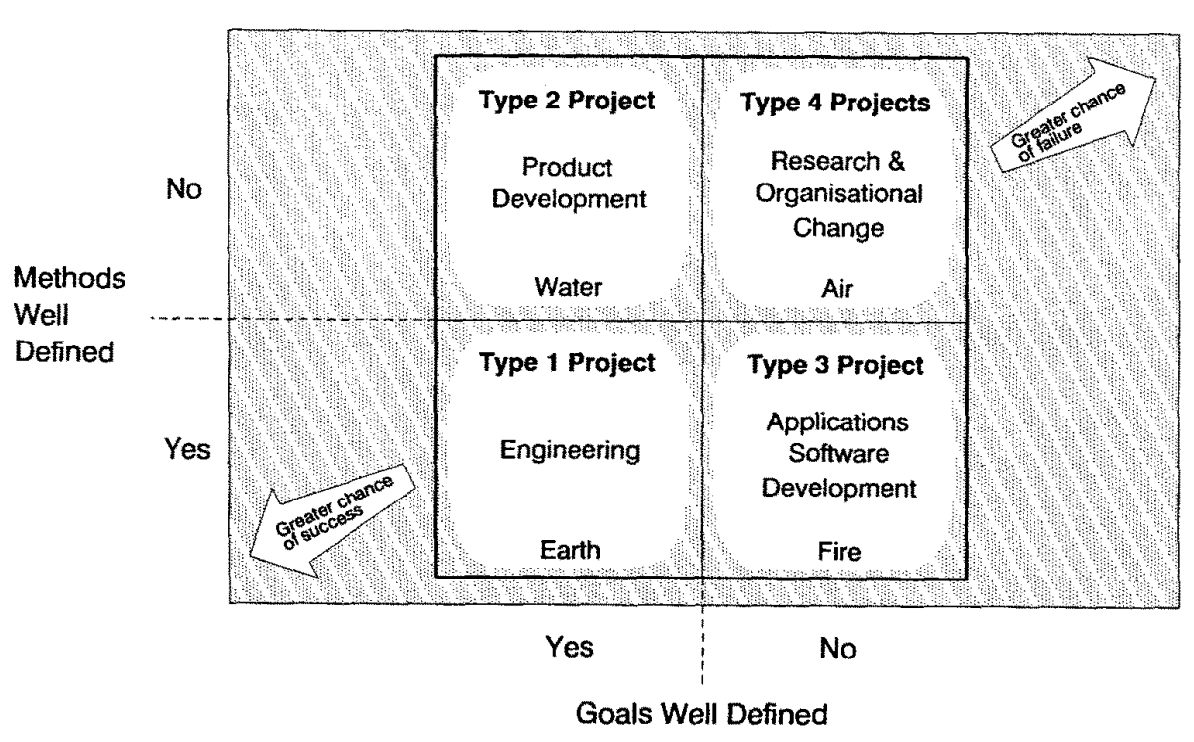
\includegraphics[width=.6\columnwidth]{figures/goal_mathods-matrix.png}
  \caption[Goals-and-methods matrix]{Goals-and-methods matrix. Reprinted from “Goals-and-methods matrix: coping with projects with ill defined goals and/or methods of achieving them,” by Turner, J.R. and Cochrane, R.A., 1993, Journal Title,International Journal of Project Management, 11(2), pp.93–102.}
  \label{fig:gmmat}
\end{figure}


Before providing an example of an actual categorisation system, the very basis of such systems should be looked at, which are the attributes that are relevant in the context of grouping projects. Many categorisation approaches that can be found in recent literature \cite<e.g., >{huemann15,turner10} are based on an empirical study by \citeA{crawford05}, which identifies 37 different attributes of categorisation that are used in project-oriented organisations. The identified attributes of this basic research, which are defined  by the authors as "the underlying characteristic that is being used to categorize projects" \cite[p. 28]{crawford05}, can be seen in Appendix B on page~\pageref{tab:cate1}. Out of the 37 attributes identified, table \ref{tab:cate2} on page~\pageref{tab:cate2} displays the ten most commonly used and the most important ones and identifies minor variations. The in the beginning of this section named motivation behind the categorisation is further supported by the result of the assessment of the organisational purposes in the scope of the research project, which ascertained as the three most named purposes 'resourcing and planning', 'matching methods to projects' and 'risk assessment' \cite{crawford05}.\\


\begin{table}[!htb]
\captionsetup{font=small}
\centering
\footnotesize
    \begin{tabular}{| l | l |}
    \hline
    {\bf Most Commonly Used Attributes} & {\bf Most Important Attributes} \\
    \hline
    1. Application area & 1. Organisational benefit \\
    2. Nature of work & 2. Cost \\
    3. Client/customer & 3. Client/customer \\
    4. Complexity & 4. Application area \\
    5. Cost & 5. Complexity  \\
    6. Size & 6. Strategic importance \\
    7. Strategic importance & 7. Risk level \\
    8. Risk level & 8. Nature of work \\
    9. Organisational benefit & 9. Resources \\
    10. Deliverables & 10. Size \\
     \hline 
    \end{tabular}
    \caption[Comparison of most common and most important attributes]{Comparison of most common and most important attributes. Adapted from Project Categorization Systems: Aligning Capability with Strategy for Better Results (p. 52), by Crawford, L., Hobbs, B. and Turner, J.R., 2005, Pennsylvania: Project Management Institute.}
\label{tab:cate2}
\end{table}


A practical approach to the categorisation of projects by organisations is constituted by multidimensional or composite systems \cite{crawford06}. Figure \ref{fig:cate}, an example for such a system, visualises the key feature of such systems, which is to combine hierarchical and parallel systems. Hierarchical systems use in the first step one parameter, for example project scope, and then apply different means for each category. Parallel systems, in contrast, make use of composite attributes to group projects. As suggested by the name, composite attributes are composed of a variation of attributes in order to be able to define more sophisticated categorisation attributes. The most common example constitutes \textit{complexity}, which can be described in organisations by using between 2 and 12 attributes. Out of these 'project scope', 'number of cites locations, countries', 'number of functions or skills', 'organisational involvement' and 'clarity of goals/objectives' are the ones organisations use the most \cite{crawford05}. \\


\begin{figure}[!hbt]
    \captionsetup{font=small}
  \centering
  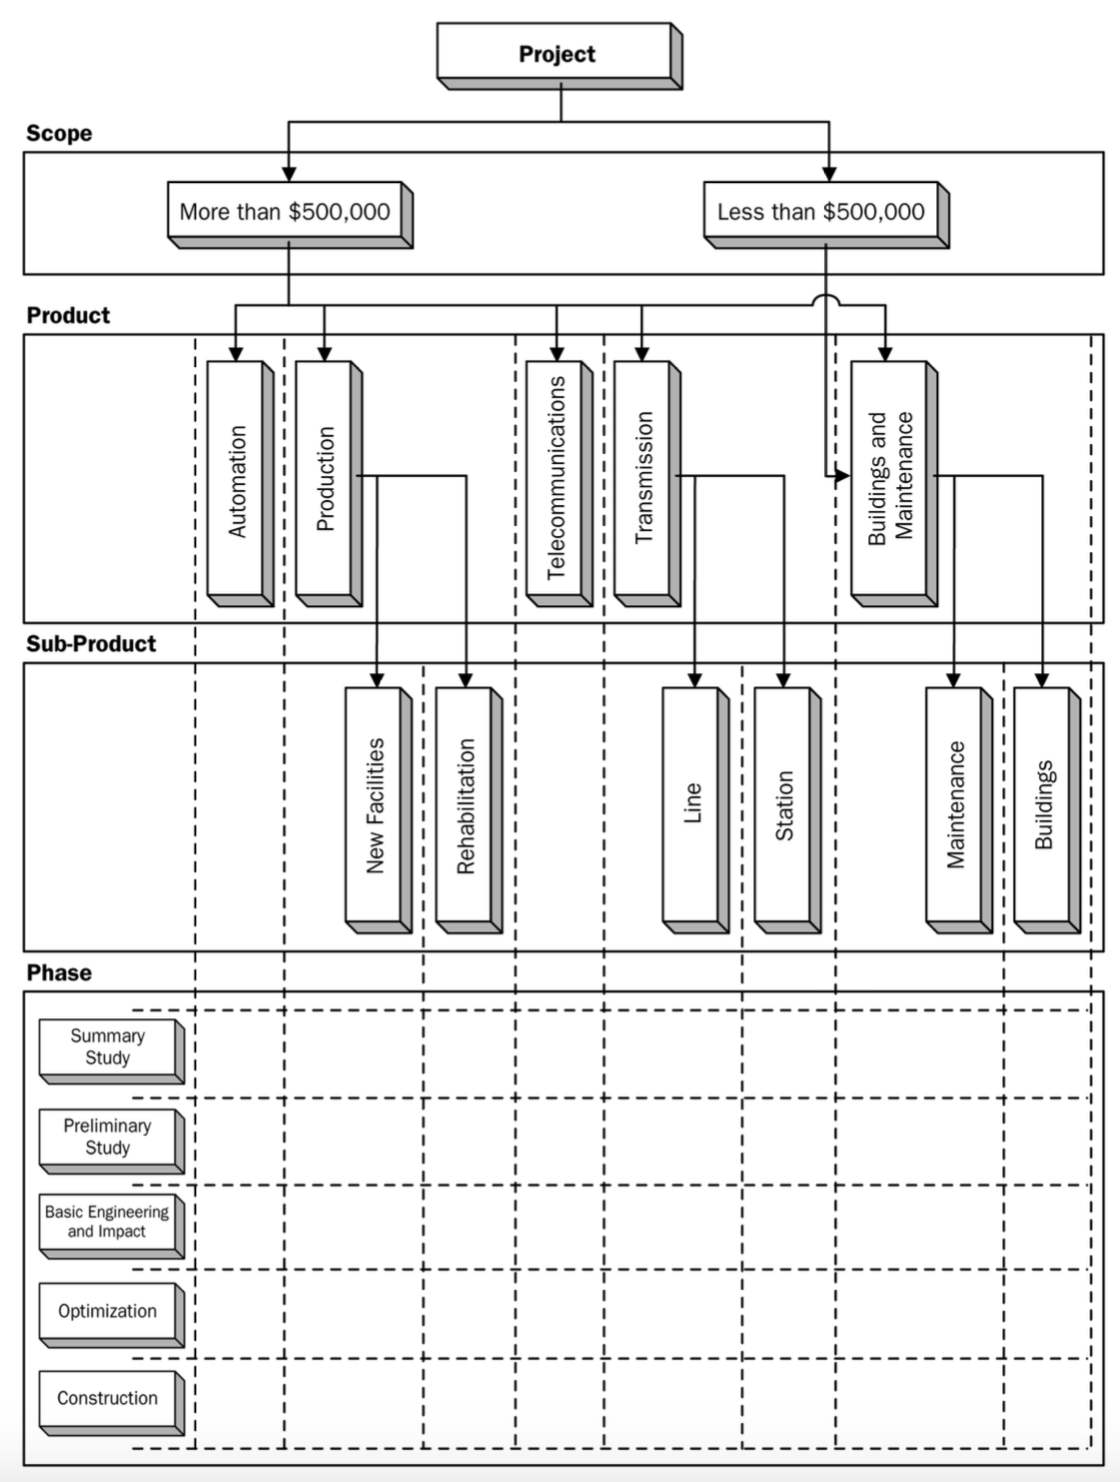
\includegraphics[width=.45\columnwidth]{figures/multidimensional_system.png}
  \caption[A hierarchical categorization with an overlay by phase]{A hierarchical categorization with an overlay by phase. Adapted from Project Categorization Systems: Aligning Capability with Strategy for Better Results (p. 33), by Crawford, L., et al., 2005, Pennsylvania: Project Management Institute.}
  \label{fig:cate}
\end{figure}


%____________________________________________________________________
\subsubsection{By project content}
The categorisation of projects by their content or, as phrased by \citeA{crawford05}  respectively their 'nature of work', is, as can be seen in table \ref{tab:cate2} on page \pageref{tab:cate2}, the \nth{2} most commonly used and the \nth{8} most important attribute. The project's content refers in this context to the very purpose of a project. For example, if a project is started to organise an event, it will incorporate tasks like programming a website, planning the all acts, etc., however, this does not mean it is a planning or an IT project, but an event project. 
A list of possible project contents adapted from \citeA{patzak17} is displayed below. 

\begin{itemize}[noitemsep]
    \item Company formation and acquisition projects
    \item Company participation projects
    \item Marketing projects, event projects
    \item Strategy projects
    \item Acquisition projects, tender projects
    \item Feasibility studies, planning projects
    \item Research projects, product development projects
    \item Organisational development projects
    \item IT projects
    \item Investment projects (construction, plant engineering, etc.)
    \item Maintenance projects, major repairs
\end{itemize}

%introducing also the categorization by archibald04


%____________________________________________________________________
\subsubsection{By project industry}
\label{sec:LiteratureRev:PCategorisation:ByPIndustry}
The application of projects in various industries has increased immensely over the past decades and since 2000 project-based work is being used in all industries and the public sector \cite{morris97, soderlund11}. Even though the categorisation by industry sector is neither ranked among the top ten most commonly used attributes, nor among the most important attributes in the results of the empirical research by \citeA{crawford05} (see table \ref{tab:cate2} on page \pageref{tab:cate2}), it is nevertheless an relevant attribute due to the fact that it is a label inherent to every project. Moreover, there is a significant correlation between industry and technology applied and based on a specific industry there can be drawn inferences about other project aspects such as common markets or project types \cite{huemann15}.
In the project management literature there can be found a variation of classifications for projects by industry-types \cite<e.g.>{wirth96, turner00}. However, since existing industries change or vanish and new industries emerge due to global phenomenons like globalisation or accelerating technological change, a potential list of industry types should be current. An example for such a collection of industries represents the following table \ref{tab:indu} on page \pageref{tab:indu} by \citeA{huemann15}. This list has its origin in the questionnaire of the before-mentioned study by \citeA[p. 148-153]{crawford05} and structures the industries by sectors.

\begin{table}[!htb]
    \captionsetup{font=small}
    \centering
    \small
    \begin{tabular}{ |l|l| }
    \hline
    {\bf Sector} & {\bf Industry} \\
    \hline
    \multirow{6}{*}{Engineering and construction} & Building \\
     & Infrastructure \\
     & Process plant \\
     & Defence \\
     & Aerospace \\
     & Environmental and waste \\ \hline
    \multirow{4}{*}{Information and telecommunications} & E-commerce \\
     & Information technology \\
     & Information systems \\
     & Telecommunications \\ \hline
    \multirow{7}{*}{Services} & Arts, entertainment, broadcasting \\
     & Recreation and sport \\
     & Business and consulting \\
     & Education and training \\
     & Financial services and insurance \\
     & Health and social services \\
     & International development \\ \hline
    \multirow{6}{*}{Industrial} & Automotive \\
     & Electronics \\
     & Manufacturing \\
     & Chemicals and pharmaceuticals \\
     & Food \\
     & Research and development \\
    \hline
    \end{tabular}
    \caption[Projects by industry type]{Projects by industry type. Adopted from Human Resource Management in the Project-Oriented Organization: Towards a Viable System for Project Personnel (p. 48), by Huemann, M., 2015, Aldershot: Gower.}
    \label{tab:indu}
\end{table}

\clearpage
%____________________________________________________________________
\subsection{Project professionals}
There doesn't exist a clear definition of the term project professional (PP) in the literature, since it was created within the scope of the research project 'careers@projects'. Nevertheless, from the perspective of its meaning, there are preexisting terms that can be used as synonyms in order to understand which project management roles are incorporated in the term project professionals.

Such a synonym represents the notion \textit{project personnel}, which is defined by \citeA[p. 76]{huemann15} in the context of the project-oriented organisation as "those human resources who need to draw on project management competency to fulfil their roles [...]". Apart from the general definition, it is important to differentiate project management personnel from the other types of personnel in the project-oriented organisation, management personnel and expert personnel. Management personnel, for instance line managers or department heads, have not only management responsibility, but also personnel authority and live off their management competencies. On the other hand, expert personnel contribute their competencies in order to fulfil their roles, such as functional or technical competencies. Another important differentiating factor of project personnel from other types of personnel in the project-oriented organisation is their contractual situation. According to \citeA{keegan03}, up to 80 per cent of personnel in projects has temporary contracts compared  to only between 20 and 40 per cent of personnel in the project-oriented organisations and compared to 11.2 per cent in all OECD countries in 2017 \cite{OECD17}. This aspect is on of the reasons for the rising significance of project-based work, as in times of accelerating change, agility and flexibility become more and more important. Apart from the contractual perspective, the roles incorporated in the term project personnel are crucial in order to gain a better understanding of what differentiates project personnel from other personnel in an organisation. \citeA{huemann15} defines the scope wider as she not only includes personnel working directly in a particular project, but also personnel of the project-oriented organisation, which is frequently engaged in projects and as a result become "members of project organisation in particular roles."

In summary, this means firstly, that the roles incorporated in the two terms include apart from project managers, also project team members, the project team, project contributors and project owners. Characteristics of each of the roles can be seen in table \ref{tab:roles} on page \pageref{tab:roles} Secondly, what can be derived from that, is that project personnel may have, despite their role in one or multiple projects, also a role in the permanent organisation, which will be especially relevant when it comes to the analysis of the outcomes of the study \cite{huemann15}.

\begin{sidewaystable}
\captionsetup{font=scriptsize}
\centering
\tiny
    \begin{tabularx}{22cm}{X X X X X X r}
        
        \hline
        \textbf{Characteristics} & 
        \textbf{Project owner} & 
        \textbf{Project manager} & 
        \textbf{Project team member} & 
        \textbf{Project team} & 
        \textbf{Project contributor} &
         \\ 
        
        \midrule
        \textbf{Names} & 
        \begin{itemize}[noitemsep,topsep=0pt, leftmargin=0pt]
            \item Project owner, project sponsor, project steering committee, project supervisory board, etc. 
        \end{itemize} & 
        \begin{itemize}[noitemsep,topsep=0pt, leftmargin=0pt]
            \item Project manager, project leader, project co-ordinator, project director etc. 
        \end{itemize} & 
        \begin{itemize}[noitemsep,topsep=0pt, leftmargin=0pt]
            \item Project team member, project core team member, project management team member, project engineer, etc. 
        \end{itemize} & 
        \begin{itemize}[noitemsep,topsep=0pt, leftmargin=0pt]
            \item Project team, project management team 
        \end{itemize} & 
        \begin{itemize} [noitemsep,topsep=0pt, leftmargin=0pt]
            \item Project contributor; expert, project worker etc. 
        \end{itemize} & 
         \\
             
        \textbf{Importance for project success}  & 
        \begin{itemize} [noitemsep,topsep=0pt, leftmargin=0pt]
            \item Very high 
        \end{itemize} & 
        \begin{itemize} [noitemsep,topsep=0pt, leftmargin=0pt]
            \item Very high 
        \end{itemize} & 
        \begin{itemize} [noitemsep,topsep=0pt, leftmargin=0pt]
            \item High 
        \end{itemize} & 
        \begin{itemize} [noitemsep,topsep=0pt, leftmargin=0pt]
            \item Very high 
        \end{itemize} & 
        \begin{itemize} [noitemsep,topsep=0pt, leftmargin=0pt]
            \item High 
        \end{itemize} & 
         \\
        
        \textbf{Objectives} & 
        \begin{itemize} [noitemsep,topsep=0pt, leftmargin=0pt]
            \item Realization of project-related organization interests, 
            \item Strategic project management
            \item Provision of context information relevant for project
        \end{itemize} & 
        \begin{itemize} [noitemsep,topsep=0pt, leftmargin=0pt]
            \item Realization of project interests
            \item Strategic and operative project management
            \item Ensuring project information 
        \end{itemize} & 
        \begin{itemize} [noitemsep,topsep=0pt, leftmargin=0pt]
            \item Fulfilling work packages
            \item Possibly leading a sub-team
            \item Participating in project team meetings
            \item Contributing to project management and project marketing 
        \end{itemize} & 
        \begin{itemize} [noitemsep,topsep=0pt, leftmargin=0pt]
            \item Developing the “Big project picture” 
            \item Ensuring synergies 
            \item Solving conflicts 
            \item Ensuring commitment 
            \item Organizing learning in the project 
        \end{itemize} & 
        \begin{itemize} [noitemsep,topsep=0pt, leftmargin=0pt]
            \item Contributing to work packages
            \item Participating in sub team meetings 
        \end{itemize} &
         \\
        
        \textbf{Non-objectives} & 
        \begin{itemize} [noitemsep,topsep=0pt, leftmargin=0pt]
            \item Performance of the tasks of the project manager
            \item Arbitrator for the project team 
        \end{itemize} & 
        \begin{itemize} [noitemsep,topsep=0pt, leftmargin=0pt]
            \item Only work on the project content
            \item Expert on the project content 
        \end{itemize} & 
        \begin{itemize} [noitemsep,topsep=0pt, leftmargin=0pt]
            \item Only tasks as expert 
        \end{itemize} & 
        \begin{itemize} [noitemsep,topsep=0pt, leftmargin=0pt]
            \item Individual work 
        \end{itemize} & 
        \begin{itemize} [noitemsep,topsep=0pt, leftmargin=0pt]
            \item Participating in project team meetings  
        \end{itemize} & 
         \\
        
        \textbf{Number of persons} & 
        \begin{itemize} [noitemsep,topsep=0pt, leftmargin=0pt]
            \item One (for small projects) or two to maximum four (for larger projects)
            \item Same or higher levels in the hierarchy 
        \end{itemize} & 
        \begin{itemize} [noitemsep,topsep=0pt, leftmargin=0pt]
            \item One person
            \item In practice sometimes two persons 
        \end{itemize} & 
        \begin{itemize} [noitemsep,topsep=0pt, leftmargin=0pt]
            \item One person 
        \end{itemize} & 
        \begin{itemize} [noitemsep,topsep=0pt, leftmargin=0pt]
            \item 3 – 12 persons 
        \end{itemize} & 
        \begin{itemize} [noitemsep,topsep=0pt, leftmargin=0pt]
            \item One person 
        \end{itemize} & 
         \\
        
        \textbf{Competencies} & 
        \begin{itemize} [noitemsep,topsep=0pt, leftmargin=0pt]
            \item Industry Company/organization
            \item Project management
            \item Strategic orientation and decision-making abilities
            \item Social competence 
        \end{itemize} & 
        \begin{itemize} [noitemsep,topsep=0pt, leftmargin=0pt]
            \item Project management
            \item Company/organization
            \item Industry
            \item Product
            \item Social competence 
        \end{itemize} & 
        \begin{itemize} [noitemsep,topsep=0pt, leftmargin=0pt]
            \item Expert 
            \item Project management
            \item Social competence 
        \end{itemize} & 
        \begin{itemize} [noitemsep,topsep=0pt, leftmargin=0pt]
            \item Team work competence, project management competence 
        \end{itemize} & 
        \begin{itemize} [noitemsep,topsep=0pt, leftmargin=0pt]
            \item Expert
            \item Minimum understanding of project management 
            \item Social competence 
        \end{itemize} & 
         \\
        
        \textbf{Recruiting} & 
        \begin{itemize} [noitemsep,topsep=0pt, leftmargin=0pt]
            \item Managers affected by the project results 
        \end{itemize} & 
        \begin{itemize} [noitemsep,topsep=0pt, leftmargin=0pt]
            \item PM expert pool 
            \item Sometimes: external market 
        \end{itemize} & 
        \begin{itemize} [noitemsep,topsep=0pt, leftmargin=0pt]
            \item Expert pool (or department)
            \item Sometimes: external market 
        \end{itemize} & 
        \begin{itemize} [noitemsep,topsep=0pt, leftmargin=0pt]
            \item Is temporary, thus needs to be developed on a project
        \end{itemize} & 
        \begin{itemize} [noitemsep,topsep=0pt, leftmargin=0pt]
            \item Expert Pool (or a department) 
            \item External market 
        \end{itemize} &
         \\    

    \bottomrule 
    \end{tabularx}
    
    \caption[Overview on roles of project personnel]{Overview on roles of project personnel. Adopted from Human Resource Management in the Project-Oriented Organization: Towards a Viable System for Project Personnel \\ (p. 85), by Huemann, M., 2015, Aldershot: Gower.}
    \label{tab:roles}
\end{sidewaystable}


\subsection{Summary of the literature}
This chapter showed that in the project management field, which is a relatively young research field \cite{Uchitpe16}, there is still room for researching basic concepts. Furthermore it provided a theretical basis for the subsequent chapters, which is crucial for this thesis as in order to apply the developed models on the obtained qualitative data sets a lucid definition of the terms is inalienable. The demarcations of the terms project content and project industry are thereof especially relevant, as they constitute the pillars of the main working model. However, also the term project professional is relevant, since during the analysis process of the subject's careers it has to be identified, whether the interviewee was involved in project-related work at all. Now, after having set this notional framework, in the subsequent chapter the working model will be introduced.

